%     ApJ article: Wreathes of Magnetism in Rapidly Rotating Suns
%     
%     Serious Beginning: June, 2008 (at KITP)
%     Target Completion date : Sep, 2008
%     Submitted :  May 26, 2009
%
%     Benjamin Brown
%
%     Now using AASTex style sheets

\chapter{Cyclic Dynamo Action Achieved at $5\thinspace\Omega_\odot$}
\label{chapter:case D5}
\label{sec:oscillating_dynamo}
Our more rapidly rotating simulation, case~D5 at five times
the current solar rate, also builds strong wreaths of magnetism that
span the convection zone.  However, in this simulation the dynamo is not steady
in time and instead goes through cycles of activity.  During a cycle,
the global-scale magnetic fields wax and wane in strength and at the
lowest field strengths they can flip their polarity.
We shall begin by looking at the general properties of the convective
flows and their associated differential rotation and meridional
circulation, and then turn to examining the nature of the magnetic
fields and their time-varying behavior.


\section{Patterns of Convection in Case~D5}

\begin{figure}
  \begin{center}
    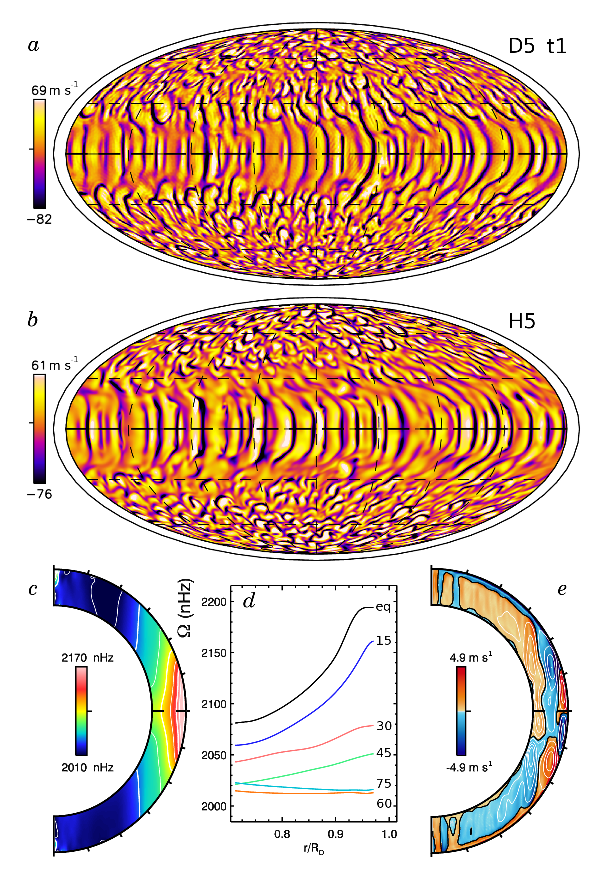
\includegraphics[width=0.7\linewidth]{figs/chapter_6/Figure_6/Figure_6.eps}
  \end{center}
  \caption[Patterns of convection in case~D5]
     {Patterns of convection in case~D5.  This simulation is rotating
     at five times the solar rotation rate.  
     $(a)$~Radial velocity $v_r$ in Mollweide projection at
     $0.95R_\odot$ for case~D5. This snapshot samples day 3880 (time t1)
     when the magnetic fields are strong.  $(b)$~Companion hydrodynamic
     case~H5, whose stronger differential rotation shears out convective
     structures in the mid-latitudes.  $(c)$~Profile of mean angular
     velocity $\Omega(r,\theta)$ for case~D5, with $(d)$~radial cuts of
     $\Omega$ at selected latitudes.  $(e)$~Meridional circulations for
     case~D5, with magnitude and sense of circulation indicated by color
     (red counter-clockwise, blue clockwise) and streamlines of mass flux
     overlaid.
  \label{fig:case_D5_patterns}}
\end{figure}

Figure~\ref{fig:case_D5_patterns}$a$ shows a snapshot of the patterns
of convection realized in case~D5 near the top of the domain.
Much as in the radial velocity patterns shown for case~D3 
(Figs.~\ref{fig:case_D3_patterns}$a$,\ref{fig:case_D3_many_depths}$e$),
here with faster rotation we continue to have prominent
north-south aligned cells in the lower latitudes and more isotropic
patterns near the poles.  There is some modulation with longitude in
the equatorial roll amplitudes.  The downflows are fast and narrow,
while the upflows are broader and slower.  The convection establishes
a prominent differential rotation, with a fast equator and slow poles
(Fig.~\ref{fig:case_D5_patterns}$c$).

As in case~D3, here too the convective downflow structures propagate
more rapidly than the differential rotation in which they are embedded.
In the equatorial band, these structures move in
a prograde fashion and at high latitudes in the retrograde sense.  In
the polar regions, the radial velocity patterns have a somewhat cuspy
appearance, with the strongest downflows appearing to favor the
westward and lower-latitude side of each convective cell.  This may be
a consequence of the strong retrograde differential rotation in those
regions.  


The convective structures are quite similar to those realized in the
hydrodynamic case~H5 (Fig.~\ref{fig:case_D5_patterns}$b$), though
there are some noticeable differences, particularly at the mid
latitudes (around $\pm30^\circ$).  In the hydrodynamic case there is
little radial flow in these regions, as the strong differential
rotation shears out the convective cells.  This region is
equatorward of the tangent cylinder, an imaginary boundary tangent to
the base of the convection zone and aligned with the rotation axis.
For rotating convective shells, it has generally been found that the
dynamics are different inside and outside the tangent cylinder, due to
differences in connectivity and rotational constraint in these two
regions \citep[e.g.,][]{Busse_1970}.  The tangent cylinder in our geometry
intersects with the stellar surface at roughly $\pm42^\circ$ of
latitude.  In our compressible simulations, we generally find that the
convective patterns in the equatorial regions are bounded by a conic
surface rather than the tangent cylinder \citep{Brown_et_al_2008}.  In
case~H5 the strong differential rotation serves to disrupt the
convection at the mid-latitudes.  In contrast, in the dynamo case~D5
the differential rotation is substantially weaker in both radial and
latitudinal angular velocity contrasts
(Table~\ref{table:delta_omega}).  As is evident in
Figure~\ref{fig:case_D5_patterns}$a$, the convective cells fill in
this region quite completely.



The time-averaged angular velocity profile $\Omega(r,\theta)$ is shown
for case~D5 in Figures~\ref{fig:case_D5_patterns}$c,d$.   The
latitudinal angular velocity contrast $\Delta \Omega_\mathrm{lat}$ and
radial contrast $\Delta \Omega_r$ in this case is
remarkably similar in amplitude to that realized in case~D3
(Table~\ref{table:delta_omega}), even though the basic rotation rate
$\Omega_0$ is substantially faster.  This is in marked contrast to our
hydrodynamic companion cases where faster rotation leads to greater
angular velocity contrasts.  The accompanying meridional circulation patterns
for case~D5 (Fig.~\ref{fig:case_D5_patterns}$e$) appear to have three
major cells of circulation in each hemisphere.  These flows are weaker
than in case~D3.  They are very similar to the circulations found in case~H5.




\section{Oscillations in Energies and Changes of Polarity}
The dynamo action realized by the convection in case~D5 exhibits
significant changes in time.  This time-varying behavior is readily
visible as oscillations of the volume-averaged kinetic and magnetic
energy densities, as shown in Figure~\ref{fig:case_D5_energies}$a$ at
a time long after the dynamo has saturated and reached equilibration.
Here the kinetic energy of differential rotation (DRKE) undergoes
factor of five changes on periods of 500-1000 days.  As DRKE decreases
the magnetic energies increase. Moving in concert are the mean
toroidal (TME) and mean poloidal (PME) magnetic energies.  The mean
poloidal fields appear to lag slightly behind the mean toroidal fields
as they both change in strength. The fluctuating magnetic energies
(FME) track the largest rises in the mean fields but decouple during
many of the deepest dips.  In contrast, the variations in convective
kinetic energies (CKE) show little organized behavior in time, and
appear to change substantially only when the differential rotation is
highly suppressed during the period from day 7500 to day 8300.  The
energy contained in the meridional circulations (MCKE) is weaker and
not shown.  Though it varies somewhat in time, there is not a clear
relation to the changes in magnetic energies.

\begin{figure*}
%\begin{sidewaysfigure}
  \begin{center}
%    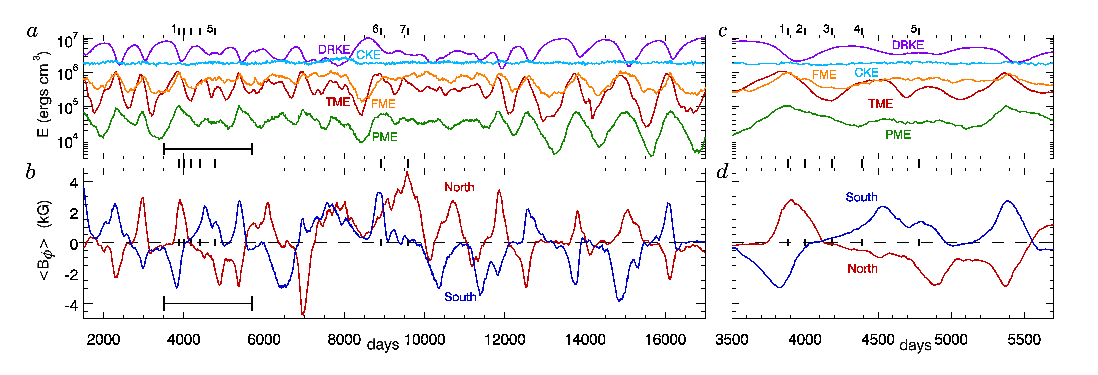
\includegraphics[width=\linewidth]{figs/chapter_6/Figure_7/Figure_7.eps}\\
    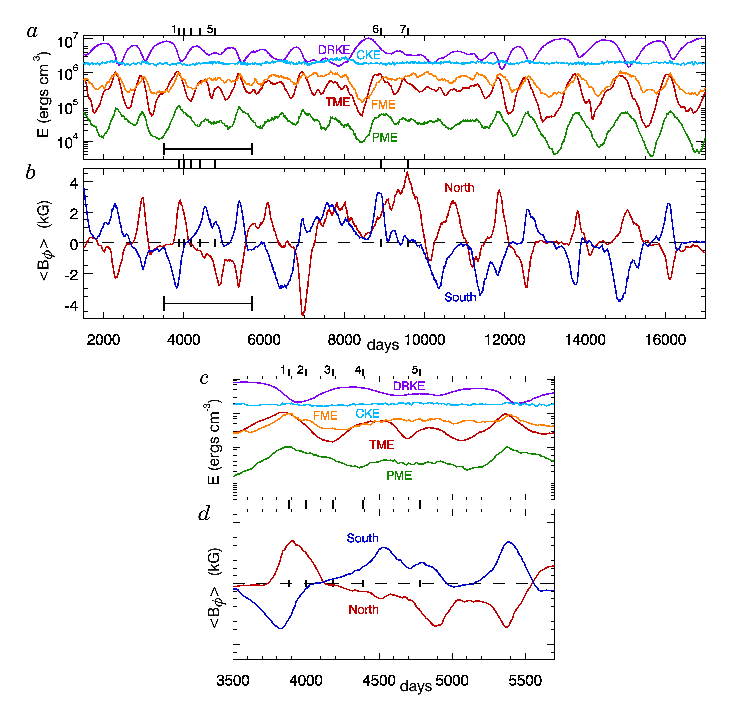
\includegraphics[width=0.8\linewidth]{figs/chapter_6/Figure_7/Figure_7b.eps}\\
  \end{center}
  % 600dpi, read in with GIMP
  \caption[Complex time evolution in case~D5 with flips in polarity of magnetic wreaths]
    {Complex time evolution in case~D5 with flips in polarity of magnetic wreaths. 
    $(a)$~Volume-averaged energy densities for kinetic
    energy of convection (CKE), differential rotation (DRKE) and for
    magnetic energy in fluctuating fields (FME), in mean toroidal fields
    (TME) and in mean poloidal fields (PME) as labeled.  Oscillations on
    roughly 500-1000 day periods are visible in the magnetic energies
    and in DRKE, though CKE stays nearly constant.  
    $(b)$~Mean toroidal field $\langle B_\phi \rangle$ averaged over entire northern and
    southern hemispheres (labeled) at mid-convection zone ($0.85 R_\sol$).
    Early in the simulation, opposite polarities dominate each
    hemisphere.  Several reversals occur, along with several extreme
    excursions which do not flip the polarity of the global-scale field.
    During the interval from roughly day 7700 to 10200, 
    the dynamo falls into peculiar single
    polarity states, with one polarity dominating both hemispheres.
    Bracketed interval from day 3500 to 5700 spans one full polarity
    reversal; $(c)$~shows volume-averaged energy densities during
    this period, and $(d)$~the mean toroidal field with same vertical
    axis scales as in $(a,b)$.   Thick labeled tick marks above $a,c$
    indicate time samples used in later images. 
    %
%    \textbf{experimental vertical layout; will expand bottom section
%    to same width.}
  \label{fig:case_D5_energies}} 
%\end{sidewaysfigure}
\end{figure*}


Magnetic energies in case~D5 can rise to be a substantial
fraction of the kinetic energies.  Averaged over the nearly 16000 days
shown here, the magnetic energies are about 17\% of the kinetic
energies.  During individual oscillations the magnetic energies can
range from a few percent of the kinetic energies to levels as high as
50\%.  The kinetic energy is largely in the fluctuating convection and
differential rotation, with CKE fairly constant and ranging from
15-60\% of the total kinetic energy as DRKE grows and subsides, itself
contributing between 40 to 85\% of the kinetic energy.  The magnetic
energies are largely split between the mean toroidal fields and the
fluctuating fields, with TME containing about 35\% of the magnetic
energy on average, FME containing about 61\% and PME containing 4\%.
The roles of these energy reservoirs change somewhat through each
oscillation.  At any one time, between 10 and 60\% of the magnetic
energy is in TME while FME contains between 30 and 85\% of the total.
Meanwhile, PME can comprise as little as 1\% or as much as 10\% of the
total.  Generally, PME is about 12\% of TME, but because PME lags the
changes in TME slightly, there are periods of time when PME is almost
40\% of TME.


The global-scale magnetic fields can reverse their polarities during
some of the oscillations in magnetic energies.  This is evident in
Figure~\ref{fig:case_D5_energies}$b$ showing
averages at mid-convection zone of the longitudinal magnetic
field $\langle B_\phi \rangle$ over the northern and southern
hemispheres.  Reversals  in field polarity occur periodically, with
typical time scales of roughly 1500 days.  These reversals appear to
happen shortly after peak 
magnetic energies are achieved, but do not occur every time magnetic
energies undergo a full oscillation.  Rather, it appears that several
failed reversals occur where the magnetic energies drop and the
average fields decline in strength, only to return with the same
polarity a few hundred days later, for each successful polarity reversal.

We focus in the following discussion on one such reversal, shown in
closeup in Figures~\ref{fig:case_D5_energies}$c,d$ and spanning the
interval of time between days 3500 and 5700.  Two reversals occur during
this interval, with the global polarities flipping into a
new state at roughly day 4100 and then changing back again at about
day 5500.  Detailed measurements of kinetic and magnetic energies
during this interval are shown in Table~\ref{table:energies}. 

\section{Global-Scale Magnetic Reversals}

The nature of the global-scale magnetic fields during the reversal
spanning days 3500-5700
are presented in detail in Figure~\ref{fig:case_D5_reversal}.  Several
samples of longitudinal magnetic field $B_\phi$ are shown at mid-convection zone spanning this
time period.  The timing of these samples is indicated in
Figure~\ref{fig:case_D5_energies} by numeric labels and likewise in
Figure~\ref{fig:case_D5_reversal}$a$ which shows azimuthally-averaged
$\langle B_\phi \rangle$ in a time-latitude map that spans the
reversal.

Before a reversal, the magnetic wreaths of case~D5 are very similar
in appearance to the wreaths realized in case~D3.  They are dominated
by the azimuthally-averaged component of 
$B_\phi$, while also showing small-scale variations where convective
plumes distort the fields (Fig.~\ref{fig:case_D5_reversal}$b$).
At mid-convection zone, typical longitudinal field strengths are of
order $\pm 13$~kG, while peak field strengths there can reach $\pm 40$~kG. 
Meanwhile $\langle B_\phi \rangle$ is fairly anti-symmetric 
between the northern and southern hemispheres
(Fig.~\ref{fig:case_D5_reversal}$g$).  Shortly before a reversal, the
magnetic wreaths strengthen in amplitude and become more
anti-symmetric about the equator. 


\begin{figure}
  \begin{center}
    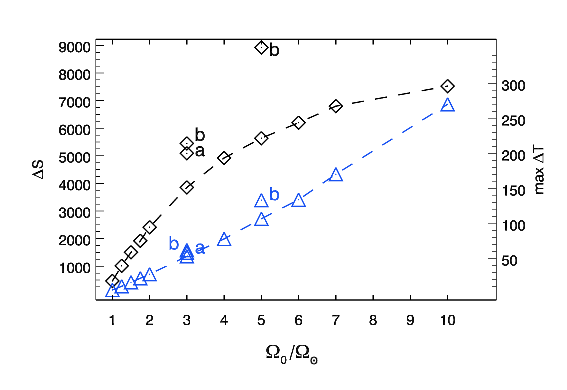
\includegraphics[width=0.55\linewidth]{figs/chapter_6/Figure_8/Figure_8.eps}
  \end{center}
  \caption[Evolution of $B_\phi$ during a polarity reversal in case~D5]
          {Evolution of $B_\phi$ during a polarity reversal in case~D5.
    $(a)$~Time-latitude plot of $\langle B_\phi \rangle$ at
    mid-convection zone.  $(b-f)$~Snapshots of $B_\phi$ in Mollweide
    projection at mid-convection zone ($0.85R_\odot$) at times
    indicated by numbers in $a$.  Between reversals the field is dominated by the
    mean component, but during reversals substantial fluctuations
    develop.  $(g-k)$~Accompanying samples of azimuthally-averaged 
    $\langle B_\phi \rangle$, showing structure of mean fields
    with radius and latitude at same instants in time.
  \label{fig:case_D5_reversal}}
% actual days: 3881.7406       3996.6234       4182.5453       4391.7875       4782.1312      
\end{figure}

They reach their peak values just before the polarity change at
roughly day 4000 but then quickly begin to unravel, gaining
significant structure on smaller 
scales (Fig.~\ref{fig:case_D5_reversal}$c$).  At the same time,
prominent magnetic structures detach from the higher-latitude edges and
begin migrating toward the polar regions.  
Meanwhile, $\langle B_\phi \rangle$  loses its anti-symmetry between
the two hemispheres, with $\langle B_\phi \rangle$ in one hemisphere
typically remaining stronger and more concentrated than in the other
(Fig.~\ref{fig:case_D5_reversal}$h$).  The stronger
hemisphere (here the northern) retains its polarity for about 100 days
as the fields in the other hemisphere (here southern) weaken and
reverse in polarity.  At this point the new wreaths of the next
cycle, with opposite polarity, are already faintly visible at the
equator. 

Within 100 days these new wreaths grow in strength and become
comparable with the structures they replace, which are still visible at
higher latitudes (Figs.~\ref{fig:case_D5_reversal}$d, i$).  The
mean $\langle B_\phi \rangle$ begins to contribute
significantly to the overall structure of the new wreaths, and soon
the polarity reversal is completed.  In the interval immediately after
the reversal, small-scale fluctuations still contribute significantly
to the overall structure of the wreaths, and $B_\phi$ has complicated
structure at mid-convection zone.  At this time, the peak magnetic
field strengths are somewhat lower, at about $\pm 20$~kG. 
As $\langle B_\phi \rangle$ becomes stronger, the wreaths return to an
anti-symmetric state, with 
similar amplitudes and structure in both the northern and southern
hemispheres (Figs.~\ref{fig:case_D5_reversal}$e,j$).  They look much
as they did before the reversal, though now with opposite polarities.
  
The wreaths from the previous cycle appear to move through the lower
convection zone and toward higher latitudes.  This can be
seen variously in the time-latitude map at mid-convection zone
(Fig.~\ref{fig:case_D5_reversal}$a$), in the Mollweide snapshots
(Figs.~\ref{fig:case_D5_reversal}$c-e$), as well as in the 
samples of $\langle B_\phi \rangle$ (Figs.~\ref{fig:case_D5_reversal}$h-j$).  
This poleward migration is likely due to hoop stresses within the
magnetic wreaths and an associated poleward-slip instability
\citep[e.g.,][]{Spruit&vanBallegooijen_1982, Moreno-Insertis_et_al_1992}.
Even at late times some signatures of the previous wreaths persist in
the polar regions, and are still visible in Figures~\ref{fig:case_D5_reversal}$e,j$ at
day 4390.  They are much weaker in amplitude than the wreaths
at the equator, but they persist until the wreaths from the next
cycle move poleward and  replace them.   As they approach the polar
regions, the old wreaths dissipate on both large and small scales, for
the vortical polar convection shreds them apart and ohmic diffusion
reconnects them with the relic wreaths of the previous cycle.

Though reversals occur on average once every 1500 days,
substantial variations can occur on shorter time scales.  
Here at mid-cycle the mean longitudinal field $\langle B_\phi \rangle$
becomes quite weak as the wreaths become concentrated in smaller
longitudinal intervals of the equatorial region (as in
Figs.~\ref{fig:case_D5_reversal}$f,k$ at day 4780).  At other times 
the mean longitudinal fields become quite asymmetric, with one
hemisphere strong and one weak (i.e.,~during days 4900-5200) before
regaining their anti-symmetric nature shortly prior to the next reversal. 




\section{Temporal Changes in Differential Rotation}
The strong magnetic fields in case~D5 suppress the
global-scale flow of differential rotation.  
As the fields themselves vary in strength, the differential rotation
responds in turn, becoming stronger as the fields weaken and then
diminishing as the fields are amplified.  These cycles of faster and
slower differential rotation are visible in the traces of DRKE shown
in Figure~\ref{fig:case_D5_energies}$a$.  
We revisit here the interval explored in closer detail both in
Figure~\ref{fig:case_D5_energies}$c$ and in
Figure~\ref{fig:case_D5_reversal}, spanning days 3500 to 5700 of the
simulation and one full polarity reversal.  

\begin{figure}
  \begin{center}
    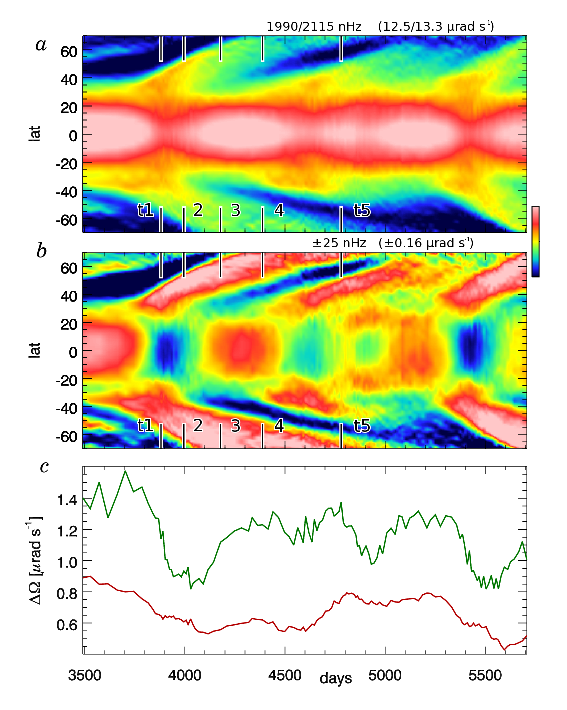
\includegraphics[width=0.8\linewidth]{figs/chapter_6/Figure_9/Figure_9.eps}
  \end{center}
  \caption[Time-varying differential rotation in case~D5] 
	  {Time-varying differential rotation in case~D5. 
    $(a)$~Time-latitude map of angular velocity $\Omega$ at
    mid-convection zone ($0.85R_\odot$).  There are substantial
    temporal variations at both the equator and high latitudes.  
    $(b)$~These are accentuated by subtracting the time-averaged
    profile of $\Omega(r,\theta)$ at each latitude.  Visible are
    poleward propagating speedup structures at high latitudes and more
    uniform modulations near the equator.
    $(c)$~Corresponding variations in $\Delta \Omega_\mathrm{lat}$
    near the surface (upper~curve, green) and at mid-convection zone
    (lower, red).
  \label{fig:case_D5_omega}}
\end{figure}

The angular velocity $\Omega$ at mid-convection zone is shown for this
period as a time-latitude map in Figure~\ref{fig:case_D5_omega}$a$.
Here again the timing marks t1--t5 refer to the snapshots of $B_\phi$
shown in Figures~\ref{fig:case_D5_reversal}$b-k$.
In the equatorial regions, the differential rotation remains fast and
prograde, but with some modulation in time.  Prominent structures of
speedup are visible propagating toward the poles at the high
latitudes.   These structures are much more evident when we subtract
the time-averaged profile of $\Omega$ for this period at each
latitude (Fig.~\ref{fig:case_D5_omega}$b$).  They appear as strong,
tilted fast (red) structures extending from roughly $\pm30^\circ$
latitude poleward.  In the northern hemisphere, three such structures
are launched over this interval.  In contrast, in the south only two
such structures are evident.  One is perhaps launched around day 4500
but does not survive or propagate.  Comparing these features with the
propagation of magnetic fields shown in
Figure~\ref{fig:case_D5_reversal}$a$ over the same interval, we find
that velocity speedup features are well correlated with the poleward
migration of mean longitudinal magnetic field.
The velocity features bear some resemblance to the poleward
branch of torsional oscillations observed in the solar convection
zone over the course of a solar magnetic activity cycle, though on a
much shorter time scale here as befits the correspondingly shorter time
between magnetic polarity reversals in these dynamo simulations.  

These velocity features propagate toward the poles relatively
slowly.  In a period of roughly 500 days they travel about $40^\circ$
in latitude, or a distance of about 410~Mm.  Their propagation
velocity is about $0.8~\mathrm{Mm}\thinspace\thinspace\mathrm{day}^{-1}$ or about 
$9~\ms$.  This is considerably slower than
the fluctuating latitudinal flows associated with the convection which
at this depth have peak speeds of $\pm 200~\ms$
during this time period.  The meridional circulations have
amplitudes of about $\pm 6~\ms$ here but do
not have a latitudinal structure at all similar to the pattern
propagation.   
The propagation speed of the speedup patterns is closer to the Alfv\'en
velocity of the mean latitudinal magnetic fields, namely
\begin{equation}
  v_{A,\theta} = \frac{\langle B_\theta \rangle}{\sqrt{4 \pi \bar{\rho}}}.
\end{equation}
At mid-convection zone the mean density is about
$0.065~\mathrm{g}\thinspace\thinspace\mathrm{cm}^{-3}$ and $\langle B_\theta \rangle$ in
the poleward propagating plumes ranges between roughly $\pm 1.5$~kG,
yielding Alfv\'en velocities of about $\pm 17~\ms$.   
This poleward migration may also be due to a poleward-slip instability
arising from the strong toroidal fields.  In this scenario, if we
neglect rotation and turbulent pumping in latitude \citep[e.g.,][]{Moreno-Insertis_et_al_1992,Jouve&Brun_2009}, the
propagation speed should be approximately the Alfv\'en velocity of the
mean toroidal magnetic fields, or about $\pm
45~\ms$ based on a mid-convection zone $B_\phi$
of approximately $\pm 4$~kG in the propagating features.  
If the poleward-slip instability is
occurring, the velocity speedup features may result from conservation
of angular momentum in the plasma that travels poleward with the wreaths.
Rotation is likely to partially stabilize wreaths against poleward-slip
\citep{Moreno-Insertis_et_al_1992},  and this may help explain their
slower poleward propagation.  
The leaky topology of the wreaths will allow plasma to
escape these structures, and this may modify the rate of their 
poleward propagation.  The weak propagating features seen in
case~D3 (Fig.~\ref{fig:case_D3_DR}) required nearly 700~days to
propagate a similar distance in latitude.  This difference may be due
to the somewhat lower magnetic field strengths achieved in that dynamo.

With the expanded sensitivity of Figure~\ref{fig:case_D5_omega}$b$, 
we can see that the equatorial modulation appears as fast and slow
pulses which span the latitude range of $\pm20^\circ$.  These
variations are fairly uniform across this equatorial region.  
The velocity variations at the equator do not correspond with the
equatorial propagating branch of torsional oscillations seen in the
Sun \citep{Thompson_et_al_2003}.  In the Sun, the equatorial branch
may arise from enhanced cooling in the magnetically active regions
\citep[e.g.,][]{Spruit_2003, Rempel_2006, Rempel_2007}.

\clearpage
The temporal variations of the angular velocity contrast in latitude
$\Delta \Omega_\mathrm{lat}$ is shown for this period in
Figure~\ref{fig:case_D5_omega}$c$.  At mid-convection zone (sampled by
red line) the variations in $\Delta \Omega_\mathrm{lat}$ are
modest, varying by roughly 15\%. 
Near the surface (green line) $\Delta \Omega_\mathrm{lat}$ shows more
substantial variations, with large contrasts when the fields are
strong in the magnetic cycle (prior to t1) and smaller contrasts when the
fields are in the process of reversing (t2, t3).  These near-surface
values of $\Delta \Omega_\mathrm{lat}$ are reported in
Table~\ref{table:delta_omega}, averaged over this entire period
(avg) and at points in time when the contrast is large (max,
at day~3702) and small (min, at day~4060).





\section{Sampling Many Magnetic Cycles in Case~D5}
\label{sec:long_time_D5}


The variations of angular velocities over considerably longer intervals of
time for case~D5 are shown in Figures~\ref{fig:case_D5_long_omega}$a,b$.  
Here too we see the equatorial modulation over many magnetic cycles and the
poleward propagating speedup bands.  Asymmetries between the northern
and southern hemisphere are evident at many times in different
cycles.  The latitudinal angular velocity contrasts shown in
Figure~\ref{fig:case_D5_long_omega}$c$ exhibit large variations.
Successive magnetic cycles can have distinctly different angular
velocity contrasts, and there are additional long-term modulations
that span many magnetic cycles.




\begin{figure}
  \begin{center}
    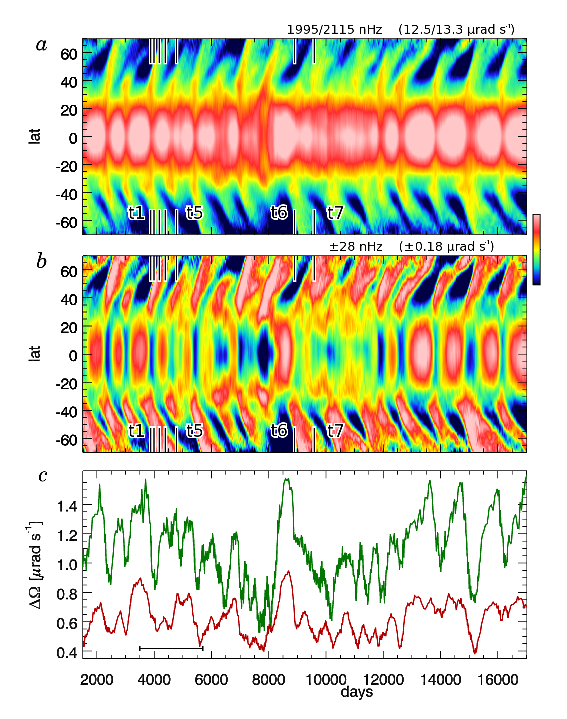
\includegraphics[width=0.8\linewidth]{figs/chapter_6/Figure_10/Figure_10.eps}
  \end{center}
  \caption[Extended history of varying differential rotation in case~D5]
	  {Extended history of varying differential rotation in case~D5. 
   $(a)$~Variations of $\Omega(r,\theta)$ at mid-convection zone.
   $(b)$~Temporal variations are emphasized by subtracting the
   time-averaged profile of $\Omega$.  Poleward propagating speedup
   structures are visible in each magnetic oscillation.
   $(c)$~Variations in $\Delta \Omega_\mathrm{lat}$ near the surface
   (upper~curve, green) and at mid-convection zone (lower, red).
  \label{fig:case_D5_long_omega}}
\end{figure}


A sampling of the associated magnetic field behavior is shown in the
time-latitude maps of $\langle B_\phi \rangle$ and  $\langle B_\theta
\rangle$ in Figures~\ref{fig:case_D5_timelat}$a,b$.  From day 1500 to
7300, four cycles occur in which wreaths of opposite polarity are
achieved in each hemisphere.  After this period, the dynamo explores
unusual single-polarity states.  Here either a single wreath
is built (t7), or two wreaths of the same polarity (t6) occupy the two
hemispheres.  After day 10700 the dynamo emerges from this state and
returns to building two wreaths of opposite polarity which flip in
their sense an additional three times as the simulation continues.

\begin{figure}[!tp]
  \begin{center}
    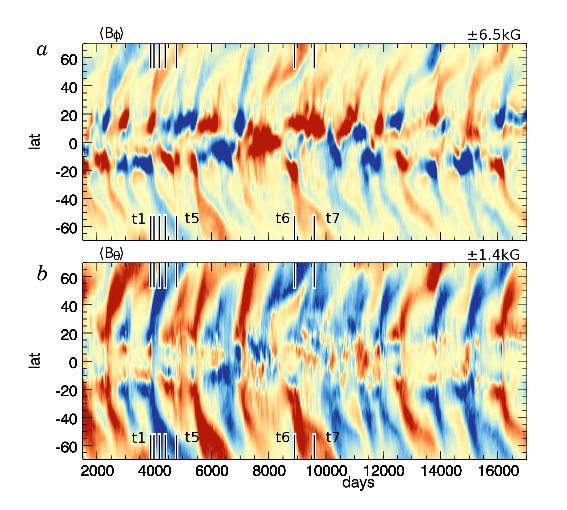
\includegraphics[width=0.8\linewidth]{figs/chapter_6/Figure_11/Figure_11.eps}
  \end{center}
  \caption[Time-latitude plots of magnetic fields in case~D5]
          {Time-latitude plots of magnetic fields in case~D5.  
	    Shown at mid-convection zone are 
    $(a)$~mean longitudinal field $\langle B_\phi \rangle$, 
    and $(b)$~mean colatitudinal field $\langle B_\theta \rangle$.
    Cycles of activity are visible, with
    fields changing polarity in the equatorial region.  Also
    prominently visible are plumes of field reaching toward the
    polar regions in a manner recalling
    Fig.~\ref{fig:case_D3_time_evolution}.  The time samples used in
    Figs.~\ref{fig:case_D5_reversal} and~\ref{fig:case_D5_single_polarity}
    are indicated.
    \label{fig:case_D5_timelat}}
\end{figure}


\clearpage
The poleward propagating magnetic features shown previously in
Figures~\ref{fig:case_D5_reversal}$a$ are evident throughout this
longer time sampling, now appearing as nearly vertical streaks in both 
$\langle B_\phi \rangle$ and  $\langle B_\theta \rangle$.  These
features continue to correlate well with the velocity speedup features
evident in Figure~\ref{fig:case_D5_long_omega}$b$.


\section{Strange States and Wreaths of a Single Polarity}
\label{sec:D5_strange_states}

These oscillating dynamos occasionally wander into distinctly
different states, and this occurs for case~D5 around day 7300.
Instead of the two nearly anti-symmetric wreaths of opposite polarity
above and below the equator, the dynamo enters a state where the
polarity in each hemisphere is the same, as shown in
Figures~\ref{fig:case_D5_single_polarity}$a,b$ at day 8903.  Here two
wreaths of same polarity occupy the two hemispheres and persist for
an interval of more than 500 days.  The positive-polarity $B_\phi$
reaches average amplitudes of 18~kG while the negative polarity
structures have average amplitudes around 3~kG.  The
azimuthally-averaged profiles of $\langle B_\phi \rangle$ emphasize
that these wreaths span the convection zone and have the same
polarity everywhere.  During this interval of time, the mean poloidal
field has changed from an odd-parity state, with strong contributions
from the odd-$\ell$ components, to an even-parity state where the
even-$\ell$ components are more prominent.

The dynamo can also achieve states where only a single wreath
is built in the equatorial regions, as in
Figures~\ref{fig:case_D5_single_polarity}$c,d$ at day 9590.  Here a
single strong wreath of positive polarity fills the northern
hemisphere, with $\langle B_\phi \rangle$ reaching a peak amplitude of
+18~kG.
This unique structure persists for about 800 days before
the dynamo flips polarity and builds a strong wreath of negative
polarity.  The predecessor of this new wreath can be seen in  
profiles of $\langle B_\phi \rangle$ where a much weaker
structure of negative polarity is visible in the lower convection zone.

\begin{figure}
  \begin{center}
    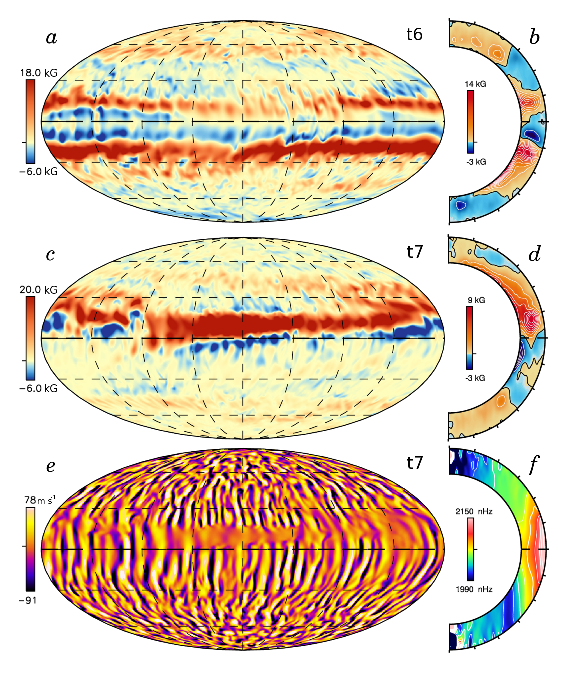
\includegraphics[width=0.8\linewidth]{figs/chapter_6/Figure_12/Figure_12.eps}
  \end{center}
  \caption[Strange single-polarity states in case~D5]
	  {Strange single-polarity states in case~D5.  
    $(a)$~Snapshot~of~$B_\phi$ at mid-convection zone, showing two
          strong wreaths of the same polarity.   
    $(b)$~Instantaneous profile of $\langle B_\phi \rangle$ at same time.
    $(c)$~Snapshot of $B_\phi$ at mid-convection zone at a time when a
    single wreath is formed.  $(d)$~Weaker negative polarity
    structures are visible in profile of $\langle B_\phi \rangle$ at
    same instant.
    $(e)$~Accompanying snapshot of $v_r$ at mid-convection zone,
    showing flows strongly affected by magnetism.  $(f)$~The
    instantaneous differential rotation, shown here as profile of
    $\Omega(r,\theta)$, is unaffected by the strong wreath.
    \label{fig:case_D5_single_polarity}}  
    % Actual days 8907.4515       9591.1937
  \vskip0.1truein
\end{figure}

The strong magnetic fields realized in the single wreath states react
back on the convective flows.  This is evident in the
accompanying snapshot of radial velocities at mid-convection zone
(Fig.~\ref{fig:case_D5_single_polarity}$e$).  In a narrow band
spanning $0-20^\circ$ latitude and coinciding with the strong tube,
the upflows and downflows have been virtually erased.
Fluctuations in $v_\phi$ and $v_\theta$ are also very small in this
region, and the flow is dominated by the streaming flows of
differential rotation.  Within the wreath the total magnetic
energy (ME) at mid-convection zone is locally about $10~\text{to}~100$
times larger than the total kinetic energy (KE), while outside the
wreath KE exceeds ME by factors of roughly $10~\text{to}~10^{4}$
at this depth. We see similar restriction of the convective
flows whenever the magnetic fields become this strong.  

The differential rotation itself
(Fig.~\ref{fig:case_D5_single_polarity}$f$) is largely
unaffected by the presence of the strong magnetic wreath.  There is no
clear signature of faster flow down the middle of the wreath.
Likewise, there is no sign of the structure in profiles of the
thermodynamic variables $P, T, S,$ or $\rho$, with the mean profile
instead dominated by latitudinal variations consistent with 
thermal wind balance. 





\section{Conclusions}

In our case~D5 the oscillations can become large, and may
result in the global-scale fields repeatedly flipping their polarity.
At times this dynamo appears to be cyclic but in other intervals it
behaves more chaotically.

The transition to richer time dependence with increasing rotation rate
in case~D5 appears to arise from subtle changes and phasing relationships
between the toroidal and poloidal magnetic production terms.  
These are difficult to assess, since the production terms themselves
are complex in space and now vary in time as well.  
It is evident that the mean poloidal fields lag the changes in the
mean toroidal fields, and there is clear migration
of magnetic field to the higher latitudes during a reversal.
This latitudinal migration may result from a polarward-slip
instability, triggered by the stronger magnetic fields that are
generated by this dynamo, and this migration may lead to the
oscillations in field strength and polarity. 
The analysis of magnetic field production that we have carried out for
case~D3 (Chapter~\ref{chapter:dynamo production}) requires
significant averaging of the turbulent correlations, accomplished there
by time averaging, to obtain a coherent picture of the balances achieved.
This has not yet been tractable for the oscillating solutions, as the
generation terms change on shorter time scales than needed to obtain
stable averages of the turbulent processes.  It appears that the
imbalances in the production and destruction of mean magnetic fields
during cyclic behavior are modest, and currently we cannot
pinpoint just which terms out of the large medley serve to drive the
oscillations. 

These dynamo oscillations are not special to case~D5. 
Indeed, we have explored a broader class of oscillating dynamo solutions,
which will be detailed in Chapter~\ref{chapter:menagerie of dynamos}.
Some of these solutions 
are realized by taking our more slowly rotating case~D3 to higher
levels of turbulence by reducing the eddy diffusivities, while
others are achieved at even higher rotation rates.  We find such
global-scale oscillations and polarity reversals fascinating, since
these appear to be the first self-consistent 3-D stellar dynamo
simulations which achieve such temporally organized behavior in the
bulk of the convection zone. 

Accompanying the oscillations in global-scale magnetic field are
changes in the differential rotation, and these signatures are the
most likely to be found through stellar observations.  The angular velocity
contrast $\Delta \Omega_\mathrm{lat}$ between the equator and high
latitudes can vary by 20\% over periods of hundreds or thousands of
days.  The patterns of speedup which we find propagating toward the
polar regions of these dynamos may have correspondence with the polar
branch of the torsional oscillations which are observed in the Sun.
The speedup features may arise from conservation of angular momentum
in fluid which is partially trapped within the wreaths as they slip
toward the poles.  The leaky nature of our wreaths will modify this
somewhat and that may explain why the wreaths are not stabilized by
rotation \citep[e.g.,][]{Moreno-Insertis_et_al_1992}.

In the next chapter, we return to our steady case~D3 to examine how
the magnetic fields are produced and maintained by the turbulent
convection and global-scale flows against resistive dissipation.






















